% !TEX root = /Users/kquine/Dropbox/Research/Papers/2015/CPS-SMT-RTSS/cps-rtss.tex


\section{SMT Solving for Distributed CPS}
\label{sec:smt-logic}

Various formal analysis problems of distributed CPSs 
can be encoded as logic formulas over the real numbers and ODEs.
%and we are interested in using SMT solving 
%to automatically check the satisfiability of those formulas.
%
The satisfiability of those formulas is undecidable for nonlinear hybrid systems  in general,
but becomes \emph{decidable} %up to any given precision $\delta > 0$ 
if we take account of robustness properties %of the system 
under numerical perturbations $\delta > 0$.
%
A \emph{$\delta$-complete decision procedure} for a formula $\phi$ returns false 
if $\phi$ is unsatisfiable, and returns true if its syntactic 
numerical perturbation of $\phi$ by bound $\delta$ is satisfiable. 
This is practically very useful since 
sampling exact values of physical parameters is not possible in reality. 

However, formulas for hybrid PALS models
may contain ODEs and universal quantification over \emph{uninterpreted real functions},
%such as  \emph{time-invariant constraints} $(\forall t.\; \psi)$.
%in order to precisely specify physical interactions between distributed components
%with clock skews and delays.
which are not supported by current state-of-the-art SMT solving techniques.
%
For example, the ODEs in $E_\mathit{Main}$ %for the main controller 
in the airplane example
include uninterpreted function symbols $\delta_L$, $\delta_V$, and $\delta_R$ for control angles.
The correspondences between  %the angles 
$(\delta_L, \delta_V, \delta_R)$ 
and the surface angles $(\alpha_L,\alpha_V,\alpha_R)$ of the subcontrollers
are given by the time-invariant constraint
$\forall t.\, (\delta_L(t) = \alpha_L(t)) \wedge (\delta_V(t) = \alpha_V(t)) \wedge (\delta_R(t) = \alpha_R(t))$.


This section shows how formulas for hybrid PALS models (presented in Section~\ref{sec:smt-encoding})
can be equivalently encoded as \emph{SMT formulas}
without the use of universal quantification over uninterpreted real functions.
For this purpose, we present a new  SMT framework to provide 
an efficient SMT algorithm
for  formulas generated from hybrid PALS models.

%\textbf{difficulties for dealing with unint. func. sym.?}
%
%A conflict-based 
%
%It is not easy to \emph{statically check without} $\delta$-complete decision procedures
%whether such subformulas of the form $\forall t \in [0,T].\; g(t) = \mathit{flow}_q(\vec{x})(t)$
%are $\delta$-consistent to each other or not.
%
%Even though two real functions
%$f_1(t)$ and $f_2(t)$ have completely different forms, 
%their corresponding formulas 
%can be consistent up to a given precision $\delta > 0$.
%E.g.,
%for $f_1(t) = \sqrt{t+1}$ and $f_2(t) = 1 + \frac{1}{2}t - \frac{1}{8}t^2 + \frac{1}{16}x^3$,
%where $f_2(t)$ is the third order taylor expansion of $\sqrt{t+1}$,
%the formulas 
%$\forall t \in [0,T].\; g(t) = f_1(t)$ and  $\forall t \in [0,T].\; g(t) = f_2(t)$
%are consistent up to precision $\delta = 0.1$ for $T = 0.8$,
%but not consistent if  $\delta = 0.01$.
%
%We need the underlying $\mathcal{T}$-solver
%to decide their consistency up to $\delta > 0$
%(e.g., by checking the unsatisfiability of the formula
%$\exists t \in [0,T].\; f_1(t) \neq f_2(t)$).


\subsection{Theory of the Real Numbers with Function Names}

SMT-based techniques for hybrid systems
normally use the standard SMT theory of the real numbers and computable %(nonlinear) 
real functions,
such as polynomials, exponentiation, trigonometric functions,  
and solutions of Lipschitz-continuous ODEs.

\begin{definition}
For a finite set $\mathcal{F}$ of computable real functions,
%(real number constants are given as $0$-ary functions).
%
$\mathcal{L}_\mathcal{F} = (\mathcal{F}, >)$ denotes the first-order signature over the real numbers
with the functions in $\mathcal{F}$,
and $\mathbb{R}_\mathcal{F} = (\mathbb{R}, \mathcal{F}^\mathbb{R}, >^\mathbb{R})$
is the standard structure of the theory of the real numbers.
\end{definition}


Solutions of ODEs are considered as \emph{atomic functions} in $\mathcal{L}_\mathcal{F}$,
and therefore the structure of ODEs cannot be used for SMT algorithms  in this logic.
This restrictive syntax makes it difficult to efficiently express logic formulas for hybrid PALS models 
in $\mathcal{L}_\mathcal{F}$. 
% which typically involve different local physical environments interacting with each other.
%Therefore, 
We present a new SMT theory,
by extending $\mathcal{L}_\mathcal{F}$, that allows to express solutions of ODEs in a modular way,
so that the size of the formula can be much reduced.


We consider a \emph{two-sorted} first-order logic with sorts $\mathit{Real}$ and $\mathit{Name}$,
where $\mathit{Real}$ denotes the real numbers,
and $\mathit{Name}$ denotes \emph{name constants} 
for unary functions composed of the functions in $\mathcal{F}$.
For example, given $\{1, +, \times, \sin, x, y\} \subset \mathcal{F}$
and two name constants $\mathtt{m_1}$ and $\mathtt{m_2}$ of sort $\mathit{Name}$,
we can have two \emph{named} real functions:
$[\mathtt{m_1}]:
(\sin(x(t)) :\mathit{Real} \to \mathit{Real})$
and
$[\mathtt{m_2}]:
([y(t) + 1, z(t)^2] :  \mathit{Real} \to \mathit{Real}^2)$.


The new logic 
includes
a collection of \emph{application operators} $\mathit{app}^n : \mathit{Name} \times \mathit{Real} \to \mathit{Real}^n$
that connect a name constant to its underlying function with range $\mathit{Real}^n$, e.g.,
\[
\mathit{app}^1(\mathtt{m_1}, 3) \equiv \sin(x(3)),
\quad
\mathit{app}^2(\mathtt{m_2}, u) \equiv [y(u) + 1,z(u)^2].
\]
%These operators ensure that each name object is really related to a concrete unary real function with domain $\mathbb{R}$.
 

In the new logic,  we take into account
a collection of \emph{integral operators} 
$\mathit{int}^{k_1,\ldots,k_n} :  \mathit{Real} \times \mathit{Name}^n  \to \mathit{Real}^{\sum_{i=1}^n k_i}$.
An integral term
$\mathit{int}^{k_1,\ldots,k_n}(u,\nu_1,\ldots,\nu_n)$
takes time value $u$
and a list of name constants $\nu_1,\ldots,\nu_n$,
to respectively denote real functions $f_1,\ldots,f_n$ with ranges $\mathit{Real}^{k_1},\ldots,\mathit{Real}^{k_n}$,
and returns the value $\int_0^u \, [f_1(t),\ldots,f_n(t)] \,\mathrm{d}t$.  
For example:
\begin{align*}
\mathit{int}^{2}(1, \mathtt{m_2}) 
&\equiv
\int_0^1
[y + 1, z^2]
\mathrm{d}t,
\\
\mathit{int}^{1,2}(T,\mathtt{m_1},\mathtt{m_2}) 
&\equiv
\int_0^T
[\sin(x),y + 1,z^2]
\mathrm{d}t.
\end{align*}









\begin{definition}
For a  set $\mathcal{N}$ of name constants
and a set  $\mathcal{O}$ of operators  $\mathit{app}^n$ and  $\mathit{int}^{k_1,\ldots,k_n}$,
the first order signature is given by 
$\mathcal{L}_{\mathcal{F}\cup\mathcal{N}} = (\mathcal{F} \cup \mathcal{N} \cup \mathcal{O}, >)$.
%
The first order structure is given by
$\mathbb{R}_{\mathcal{F}\cup\mathcal{N}} 
= (\mathbb{R} \cup N, \mathcal{F}^\mathbb{R} \cup \mathcal{N}^N \cup \mathcal{O}^{N,\mathbb{R}}, >^\mathbb{R})$
for a fixed finite set $N$ of \emph{name objects},
where the interpretation $\mathcal{N}^N$ of name constants and 
the interpretation $\mathcal{O}^{N,\mathbb{R}}$ of application and integral operators 
are given as explained above.
%
The syntax and semantics of $\mathcal{L}_{\mathcal{F}\cup\mathcal{N}}$-formulas 
is defined by means of $\mathcal{L}_{\mathcal{F}\cup\mathcal{N}}$ and $\mathbb{R}_{\mathcal{F}\cup\mathcal{N}}$
in the standard way.
%(The signature $\mathcal{L}_\mathcal{F}$ is a subsignature of $\mathcal{L}_{\mathcal{F}\cup\mathcal{N}}$,
%and the structure $\mathbb{R}_\mathcal{F}$ for the real numbers 
%is a substructure of $\mathbb{R}_{\mathcal{F}\cup\mathcal{N}}$).
\end{definition}




The satisfiability problems of $\mathcal{L}_{\mathcal{F}\cup\mathcal{N}}$-formulas in the new theory 
$\mathbb{R}_{\mathcal{F}\cup\mathcal{N}}$
can be reduced to ones in the standard theory $\mathbb{R}_\mathcal{F}$ at minimal cost,
provided that all $\mathit{Name}$ variables %in the formulas 
are only existentially quantified.
Consider an $\mathcal{L}_{\mathcal{F}\cup\mathcal{N}}$ formula 
$\exists \vec{n}.\; \psi(\vec{n})$, where 
$\vec{n}$ are only variables of sort $\mathit{Name}$ %in $\psi(\vec{n})$
and
$\psi(\vec{n})$ contains no quantifier for $\vec{n}$.
Since there are only a finite number of name objects in $\mathbb{R}_{\mathcal{F}\cup\mathcal{N}}$,
by using the standard SMT solving for equalities,
we can enumerate all \emph{consistent} assignments 
$\vec{n} = \overrightarrow{\mathit{name}}_1,\ldots,\vec{n} = \overrightarrow{\mathit{name}}_N$ for $\vec{n}$.
Let $\hat{\psi}_i$ be the formula obtained from $\psi(\vec{n})$
by replacing each name by its related function according to the $i$-th assignment $\vec{n} = \overrightarrow{\mathit{name}}_i$.
Then, $\vee_{i=1}^N \hat{\psi}_i$ is an ordinary $\mathcal{L}_\mathcal{F}$ formula
whose satisfiability can be decided by %existing SMT techniques, such as 
$\delta$-complete decision procedures. Therefore:


\begin{theorem}
The satisfiability of $\mathcal{L}_{\mathcal{F}\cup\mathcal{N}}$ formulas of the form $\exists \vec{n}.\; \psi(\vec{n})$
is decidable by  $\delta$-complete SMT solving. 
\end{theorem}


%\begin{figure}
%\begin{algorithmic}
%\STATE $V\gets$ AllUnigramsInTraining($D$)
%\STATE $N\gets$ NumberOfTweets($D$)
% \FORALL{$c \in C$}
%  \STATE $N_c \gets$ Number of tweets in Class $c$
%  \STATE ...
%  \STATE $Tweets_c \gets $All Tweets in class $c$
%  \FORALL{$t \in V$}
%    \STATE $T_ct$ = No. of times term $t$ appeared in $Tweets_c$
%  \ENDFOR
%  \FORALL{$t \in V$}
%    \STATE ...
%  \ENDFOR
%\ENDFOR
%\end{algorithmic}
%\end{figure}


%We first find a truth assignment for the names, and 
%replace names in ODEs by them
%We have a truth assignment that includes only $\mathcal{L}_\mathcal{F}$-terms.
%The satisfiability of such $\mathcal{L}_\mathcal{F}$-assignments
%can then be decided by using $\delta$-decision procedures as usual.





\subsection{SMT Encoding of Hybrid PALS Models}


We now show how hybrid PALS models
are encoded in the new SMT logic $\mathcal{L}_{\mathcal{F}\cup\mathcal{N}}$
without the use of uninterpreted real functions and universal quantification.
The idea is to construct a \emph{global} ODE formula $\phi_{\mathit{ODE}}$
that defines the combined systems of ODEs for all physical environments
in $\mathcal{E} \restriction_{\Pi} E_\mathcal{E}$.
The formula $\phi_{\mathit{ODE}}$ is parameterized by the behaviors of 
the subcomponents by means of integral operators and \emph{name variables}.
The behavior of each subcomponent $M_j \restriction E_{M_j}$ is then
specified in a modular way by assigning to each name variable an appropriate name constant for $M_j \restriction E_{M_j}$.

%First, 
We restrict our attention to time-invariant constraints \emph{with only equality terms},
such as one for the airplane example,
since physical correlations for CPS can be expressed using equality conditions in practice.
Equality  constraints, such as $x_1(t) = x_2(t)$,  can be removed
from the formula  by replacing one side with another, e.g., by replacing $x_1$ with  $x_2$.
From now on we assume that time-invariant constraints are already removed from the formula 
by this process.



Suppose that 
the formula $\phi_{\mathcal{E} \restriction_{\Pi} E_\mathcal{E}}^{T,i}$ for $\mathcal{E} \restriction_{\Pi} E_\mathcal{E}$
includes $N$ terms  to obtain a value of some parameter of $E_{M_j}$ of the form $\vec{x_j}(u)$.
We only need to use ODEs for finding those values %of all such terms
to determine the satisfiability of $\phi_{\mathcal{E} \restriction_{\Pi} E_\mathcal{E}}^{T,i}$.
A global ODE formula $\phi_{\mathit{ODE}}$
is defined as a conjunction of $N$ ODEs for such $N$ access timings,
which include all sampling and response times for each (decelerated) subcomponent in a global round.
% of $\mathcal{E} \restriction_{\Pi} E_\mathcal{E}$.

\begin{definition}
Let $\vec{t} = \{t_0,t_1,\ldots,t_N\}$ for  $N$ time variables with
$iT = t_0 \leq t_1 \leq t_2 \leq \cdots \leq t_N = (i+1)T$.
For name variables $\vec{f} = \{f_j^1,\ldots,f_j^N\}_{j \in J_S \cup J_F}$ and
global value variables $\vec{g} = \{\vec{g}_0,\ldots,\vec{g}_N\}$,
$\phi_{\mathit{ODE}}(\vec{f},\vec{t},\vec{g})$ is the %$\mathcal{L}_{\mathcal{F}\cup\mathcal{N}}$-
formula:
\[
\bigwedge_{1 \leq i \leq N}
(
\vec{g}_{i} = \vec{g}_{i-1} + 
\mathit{int}^{\vec{l}}(t_{i} - t_{i-1}, \{f_j^i\}_{j \in J_S \cup J_F})
),
\]
where $f_j^i$ denotes $E_{M_j}$'s behavior during the interval $[t_{i-1},t_i]$,
$\vec{g}_i$ denotes the values of all the physical parameters of $\mathcal{E} \restriction_{\Pi} E_\mathcal{E}$
at time $t_i$, and $\vec{l} = \{l_j\}_{j \in J_S \cup J_F}$ denotes the \emph{dimension}
of each $E_{M_j}$'s physical parameters $\vec{x_j} = (x_j^1,\ldots,x_j^{l_j})$.
\end{definition}



\begin{figure}
\centering
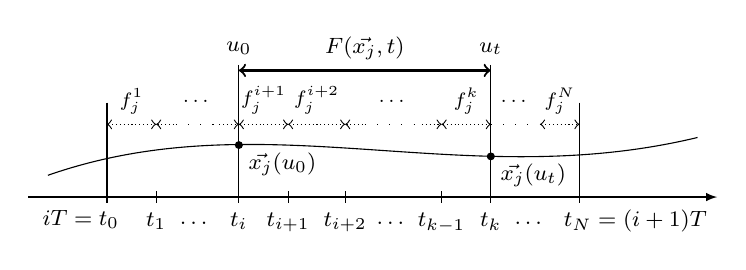
\begin{tikzpicture}[xscale=2.5,yscale=2.4,font=\footnotesize]
%baseline
\draw[-latex,thin] (-0.2,0) -- (3.3,0);

\draw[thin] (0.2,0.5) -- (0.2,-0.03) node[below,xshift=-2.2ex,yshift=0.15ex] { $iT = t_0$};
\draw[thin] (0.45,0.03) -- (0.45,-0.03) node[below] { $t_1$};
\path (0.65,-0.08) node[below] {\ldots};
\draw[thin] (1.12,0.03) -- (1.12,-0.03) node[below] { $t_{i+1}$};
\draw[thin] (1.41,0.03) -- (1.41,-0.03) node[below] { $t_{i+2}$};
\path (1.65,-0.08) node[below] {\ldots};
\draw[thin] (1.9,0.03) -- (1.9,-0.03) node[below] { $t_{k-1}$};
\path (2.35,-0.08) node[below] {\ldots};
\draw[thin] (2.6,0.5) -- (2.6,-0.03) node[below,xshift=4.7ex,,yshift=0.23ex] { $t_N = (i+1)T$};

\draw[thin] (0.87,0.7) node[above] {$u_0$}-- (0.87,-0.03) node[below] { $t_i$};
\draw[thin] (2.15,0.7) node[above] {$u_t$} -- (2.15,-0.03) node[below] { $t_{k}$};

\draw[<->,thick] (0.87,0.67) -- node[above] {$F(\vec{x_j},t)$} (2.15,0.67);

\begin{scope}[font=\scriptsize,yshift=-0.1ex]
\draw[<->,densely dotted] (0.2,0.40) -- node[above] {$f_j^1$} (0.45,0.40) ;
\draw[<-,densely dotted] (0.45,0.40) -- (0.55,0.40);
\draw[loosely dotted] (0.55,0.40) -- node[above,yshift=1ex] {\ldots} (0.77,0.40) ;
\draw[->,densely dotted] (0.77,0.40) -- (0.87,0.40);
\draw[<->,densely dotted] (0.87,0.40) -- node[above] {$f_j^{i+1}$} (1.12,0.40) ;
\draw[<->,densely dotted] (1.12,0.40) -- node[above] {$f_j^{i+2}$} (1.41,0.40) ;
\draw[<-,densely dotted] (1.41,0.40) -- (1.51,0.40);
\draw[loosely dotted] (1.51,0.40) -- node[above,yshift=1ex] {\ldots} (1.8,0.40) ;
\draw[->,densely dotted] (1.8,0.40) -- (1.9,0.40);
\draw[<->,densely dotted] (1.9,0.40) -- node[above] {$f_j^{k}$} (2.15,0.40) ;
\draw[loosely dotted] (2.15,0.40) -- node[above,yshift=1ex] {\ldots} (2.4,0.40) ;
\draw[<->,densely dotted] (2.4,0.40) -- node[above] {$f_j^{N}$} (2.6,0.40) ;
\end{scope}
\begin{scope}[yshift=0.1ex]
%\filldraw (0.2,0.19) circle (0.5pt) node[below,xshift=0.8ex] {$\vec{v}$};
\filldraw (0.87,0.26) circle (0.5pt) node[right,yshift=-1.6ex] {$\vec{x_j}(u_0)$};
\filldraw (2.15,0.2) circle (0.5pt) node[right,yshift=-1.6ex] {$\vec{x_j}(u_t)$};
%\filldraw (2.6,0.21) circle (0.5pt) node[below,xshift=1.1ex] {$\vec{v'}$};
\draw (-0.1,0.1) .. controls (1,0.5) and (2,0) .. (3.2,0.3);
\end{scope}
\end{tikzpicture}
\caption{ODE-free transformation}
\label{fig:flow-map}
\end{figure}


For any subcomponent $M_j \restriction E_{M_j}$,
an ODE subformula $\forall t \in [u_0,u_t].\; \vec{x_j}(t) = \vec{v_j} + \int_0^{t-u_0} \!  F(\vec{x_j},t)\,\mathrm{d}t$ 
in $\phi_{\mathcal{E} \restriction_{\Pi} E_\mathcal{E}}^{T,i}$
is replaced by conditions for name variables $\vec{f}$, time variables $\vec{t}$, and 
\emph{global} value variables $\vec{g}$,
as illustrated in Fig.~\ref{fig:flow-map}.
For example, if $u_0 = t_i$ and $u_t = t_k$ for some $0 \leq i \leq k \leq n$,
then all the name variables $f_j^l$ for $i \leq l < k$ are equal to 
the name constant $\mathtt{m}_{F(\vec{x_j},t)}$ for the function $F(\vec{x_j},t)$.


\begin{definition}
For an ODE formula for $M_j \restriction E_{M_j}$ of the form 
$\forall t \in [u_0,u_t].\; \vec{x_j}(t) = \vec{v_j} + \int_0^{t-u_0} \!  F(\vec{x_j},t)\,\mathrm{d}t$, 
if a name constant $\mathtt{m}_{F(\vec{x_j},t)}$ denotes the function $F(\vec{x_j},t)$,
its \emph{ODE-free} transformation is defined by the $\mathcal{L}_{\mathcal{F}\cup\mathcal{N}}$-formula:
\[
\bigvee_{0 \leq i \leq k \leq n} 
\left[
\begin{aligned}
(t_i = u_0) \wedge (t_k = u_t) \wedge \textstyle\bigwedge_{l=i}^{k-1} f^l_j \equiv \mathtt{m}_{F(\vec{x_j},t)}  ) &\wedge
\\
(\vec{x_j}(u_0) = \pi_j(\vec{g}_i) = \vec{v_j}) \wedge  (\vec{x_j}(u_t) = \pi_j(\vec{g}_k))
\end{aligned}
\right],
\]
where $\pi_j(\vec{g}_i)$ denotes $E_{M_j}$'s parameter values 
in the global parameter values $\vec{g}_i$ of $\mathcal{E} \restriction_{\Pi} E_\mathcal{E}$.
\end{definition}

Let $\mathit{tr}(\phi_{\mathcal{E} \restriction_{\Pi} E_\mathcal{E}}^{T,i})$ 
be the formula
obtained from $\phi_{\mathcal{E} \restriction_{\Pi} E_\mathcal{E}}^{T,i}$ 
by repeatedly performing this ODE-free transformation
for every ODE subformula.
Finally, we have the $\mathcal{L}_{\mathcal{F}\cup\mathcal{N}}$-formula 
$\exists (\vec{f}, \vec{t}, \vec{g}).\; \phi_{\mathit{ODE}}(\vec{f},\vec{t},\vec{g}) \wedge \mathit{tr}(\phi_{\mathcal{E} \restriction_{\Pi} E_\mathcal{E}}^{T,i})$,
which
includes neither uninterpreted real functions nor universal quantification.

\begin{theorem}
$\phi_{\mathcal{E} \restriction_{\Pi} E_\mathcal{E}}^{T,i}$
is satisfiable
iff
the $\mathcal{L}_{\mathcal{F}\cup\mathcal{N}}$-formula 
$\exists (\vec{f}, \vec{t}, \vec{g}).\; \phi_{\mathit{ODE}}(\vec{t},\vec{f},\vec{g}) \;\wedge\; \mathit{tr}(\phi_{\mathcal{E} \restriction_{\Pi} E_\mathcal{E}}^{T,i})$
is satisfiable.
\end{theorem}








